\documentclass[12pt,a4paper]{article}

% ─── kodowanie i język (XeLaTeX — natywne UTF-8) ────────────────────────────
\usepackage{fontspec}
\usepackage{polyglossia}
\setmainlanguage{polish}
\setotherlanguage{english}

% ─── matematyka ──────────────────────────────────────────────────────────────
\usepackage{amsmath,amssymb,amsthm,mathtools}

% ─── układ i typografia ──────────────────────────────────────────────────────
\usepackage[margin=2.5cm]{geometry}
\usepackage{microtype}
% lmodern not needed with fontspec
\usepackage{parskip}
\usepackage{setspace}
\setstretch{1.15}

% ─── tabele, listy, kod ──────────────────────────────────────────────────────
\usepackage{booktabs}
\usepackage{array}
\usepackage{listings}
\usepackage{xcolor}
% enumitem not available in basic installation

% ─── kolory dla kodu ─────────────────────────────────────────────────────────
\definecolor{codebg}{HTML}{F5F5F5}
\definecolor{keywd}{HTML}{0033B3}
\definecolor{comment}{HTML}{7F7F7F}
\definecolor{string}{HTML}{067D17}

\lstset{
  backgroundcolor=\color{codebg},
  basicstyle=\ttfamily\small,
  keywordstyle=\color{keywd}\bfseries,
  commentstyle=\color{comment}\itshape,
  stringstyle=\color{string},
  breaklines=true,
  frame=single,
  framesep=4pt,
  xleftmargin=8pt,
  xrightmargin=8pt,
  aboveskip=6pt,
  belowskip=6pt,
  numbers=left,
  numberstyle=\tiny\color{gray},
  numbersep=6pt
}

% ─── grafiki i rysunki ───────────────────────────────────────────────────────
\usepackage{graphicx}
\usepackage{float}
\usepackage{tikz}
\usetikzlibrary{positioning,arrows.meta}
\usepackage{subcaption}

% ─── hiperłącza ──────────────────────────────────────────────────────────────
\usepackage[hidelinks]{hyperref}

% ─── środowiska twierdzeń ────────────────────────────────────────────────────
\theoremstyle{plain}
\newtheorem{theorem}{Twierdzenie}[section]
\newtheorem{lemma}[theorem]{Lemat}
\newtheorem{corollary}[theorem]{Wniosek}
\theoremstyle{definition}
\newtheorem{definition}[theorem]{Definicja}
\newtheorem{example}[theorem]{Przykład}
\theoremstyle{remark}
\newtheorem{remark}[theorem]{Uwaga}

% ─── symbole skrótów ─────────────────────────────────────────────────────────
\newcommand{\HG}{\mathrm{HG}}
\newcommand{\rounds}{\mathrm{rounds}}
\newcommand{\popcount}{\mathrm{popcount}}
\newcommand{\view}{\mathrm{view}}
\newcommand{\mask}{\mathrm{mask}}
\newcommand{\Wval}{W_{\mathrm{valid}}}

% ─────────────────────────────────────────────────────────────────────────────
\begin{document}

% ── strona tytułowa ───────────────────────────────────────────────────────────
\begin{titlepage}
  \centering
  \vspace*{1.5cm}
  {\Large\bfseries MINI}\\[0.3cm]
  {\large Przedmiot: Gry Kombinatoryczne}\\[1.5cm]
  \rule{\linewidth}{1.5pt}\\[0.4cm]
  {\LARGE\bfseries Gra w Kapelusze na Grafach:\\[0.2cm]
  Analiza Epistemiczna, Implementacja i Dowody}\\[0.4cm]
  \rule{\linewidth}{1.5pt}\\[1.2cm]
  {\large Projekt zaliczeniowy z kodem źródłowym w C++17}\\[0.2cm]
  {\large Repozytorium: \texttt{hats} (C++17/CMake + Python/pybind11)}\\[1.5cm]
  {\large Kacper Piotrowski}\\[0.3cm]
  {\large Igor Ptak}\\[0.3cm]
  {\large 17 maja 2026}
  \vfill
\end{titlepage}

\tableofcontents
\newpage

% ─────────────────────────────────────────────────────────────────────────────
\section{Streszczenie}

Niniejszy raport analizuje kooperatywny wariant \emph{Gry w Zgadywanie Kapeluszy} (ang.\ \textit{Hat Guessing Game}) osadzony na topologiach grafowych w paradygmacie Dynamicznej Logiki Epistemicznej (DEL). Grę modelujemy jako iteracyjny protokół publicznych oznajmień na modelu Kripkego, gdzie agenci-wierzchołki widzą kapelusze wyłącznie swoich sąsiadów w grafie.

Prezentujemy autorski symulator w C++17 z powiązaniami Python/pybind11 oraz rozszerzamy go o sześć nowych topologii (\textit{ścieżka} $P_n$, \textit{akordowy cykl} $C_n^+$, \textit{hiperkostka} $Q_k$, \textit{graf kołowy} $W_n$, $K_n \setminus e$, \textit{graf dwudzielny} $K_{m,n}$) i metrykę entropii epistemicznej. Dowodzimy rygorystycznie jedenastu twierdzeń charakteryzujących dynamikę gry:

\begin{enumerate}
  \item $\rounds(K_n, w) = \min(k, n-1)$, gdzie $k = \popcount(w)$.
  \item $\rounds(C_n, w) = \infty$ dla $n \ge 4$ i każdego $w \ge 1$.
  \item $\rounds(S_n, w) < \infty$ wtw.\ $w = 1$ (samo centrum czerwone).
  \item $\rounds(P_n, w) < \infty$ wtw.\ $n \le 2$ lub ($n = 3$ i $w = 2$).
  \item $\rounds(W_n, w) < \infty$ wtw.\ $w = 2^{n-1}$ dla $n \ge 5$.
  \item $\rounds(K_n\setminus e, w) < \infty$ wtw.\ oba usunięte wierzchołki mają białe kapelusze.
  \item $\rounds(K_{m,n}, w) = \infty$ dla $m,n \ge 2$ i każdego $w \ge 1$.
  \item Graf Petersena (3-regularny, $n=10$): $\rounds = \infty$ dla wszystkich 1023 światów.
  \item $\rounds(O_n, w) < \infty$ wtw.\ $w = 1$ (tylko wierzchołek 0 czerwony); dla wszystkich $n \ge 2$.
\end{enumerate}

Eksperymenty na $C_4^+$, hiperkostkach $Q_k$, grafie Petersena i $K_{3,3}$ (graf Zagadki Trzech Mediów, powiązanej z twierdzeniem Kuratowskiego) poszerzają spektrum badanych struktur. Formułujemy kryterium gęstości wyjaśniające, dlaczego grafy rzadkie i bezskalowe zawsze kleszczą.

% ─────────────────────────────────────────────────────────────────────────────
\section{Wstęp teoretyczny i formalizacja}

\subsection{Problem i notacje}

\begin{definition}[Gra w kapelusze na grafie]
Niech $G = (V, E)$ będzie prostym grafem nieskierowanym, $V = \{0,\ldots,n{-}1\}$. Każdemu agentowi $i \in V$ przypisywany jest kolor kapelusza $c_i \in \{0,1\}$. \emph{Światem} nazywamy maskę bitową
$$w = \sum_{i=0}^{n-1} c_i \cdot 2^i \in \{1, 2, \ldots, 2^n - 1\},$$
gdzie warunek $w \ge 1$ wyraża \emph{wiedzę wspólną}, że co najmniej jeden kapelusz jest czerwony. Obserwacja agenta $i$ w świecie $w$ to
$$\view_i(w) = w \;\&\; \mask_i, \qquad \mask_i = \bigoplus_{j \in N(i)} 2^j.$$
\end{definition}

\begin{definition}[Model Kripkego dla gry]
Modelem Kripkego jest krotka $\mathcal{M} = (W, \sim_0, \ldots, \sim_{n-1})$, gdzie $W = \{1,\ldots,2^n{-}1\}$ i
$$w \sim_i w' \;\iff\; \forall j \in N(i):\; w_j = w_j'.$$
Klasa równoważności agenta $i$ dla obserwacji $v$ to $[i,v] = \{w \in W : \view_i(w) = v\}$.
\end{definition}

Relacja $\sim_i$ jest relacją równoważności (zwrotna, symetryczna, przechodnia), co zapewnia przynależność do systemu logiki epistemicznej \textbf{S5}. Aksjomat wiedzy $K_i\varphi \Rightarrow \varphi$ (T), pozytywna introspekcja $K_i\varphi \Rightarrow K_i K_i\varphi$ (4) i negatywna introspekcja (5) wynikają wprost z tego, że $\sim_i$ jest relacją równoważności na $W$.

\subsection{Protokół gry i publiczne oznajmienia}

Gra toczy się w rundach. W każdej rundzie:
\begin{itemize}
  \item \textbf{Runda odgadywania}: każdy agent $i$ z jednorodną klasą $[i, \view_i(w)] \cap \Wval$ odgaduje swój kolor.
  \item \textbf{Runda ciszy}: jeśli nikt nie odgaduje, ogłaszana jest formuła
  $\phi_t = \bigwedge_{i \in V} \neg\bigl(K_i(c_i=0) \vee K_i(c_i=1)\bigr),$
  co odpowiada przejściu do podmodelu $\mathcal{M}_{t+1} = \mathcal{M}_t|\phi_t$ poprzez usunięcie wszystkich światów, w których jakiś agent mógłby odgadnąć.
\end{itemize}

\begin{definition}[Jednorodność klasy]
Klasa $[i,v] \cap \Wval$ jest \emph{jednorodna} dla agenta $i$, gdy
$$\bigl|\{c \in \{0,1\} : \exists w' \in [i,v] \cap \Wval,\; \mathrm{bit}_i(w') = c\}\bigr| = 1.$$
Agent $i$ może odgadnąć swój kolor wtedy i tylko wtedy, gdy jego klasa jest jednorodna.
\end{definition}

\begin{definition}[Liczba rund i zakleszczenie]
$\rounds(G,w)$ oznacza łączną liczbę zdarzeń (rund odgadywania i rund ciszy) zarejestrowanych przez symulator \emph{przed} ostatecznym odgadnięciem przez wszystkich agentów. Jeśli gra się nie kończy, $\rounds(G,w) = \infty$ (zakleszczenie).
\end{definition}

% ─────────────────────────────────────────────────────────────────────────────
\section{Architektura symulatora}

\subsection{Przegląd modułów}

Kod składa się z czterech warstw (tabela~\ref{tab:layers}):

\begin{table}[h]
\centering
\caption{Moduły symulatora HATS}
\label{tab:layers}
\begin{tabular}{lll}
\toprule
Warstwa & Pliki & Odpowiedzialność \\
\midrule
Typy & \texttt{types.hpp} & \texttt{WorldMask, VertexMask} jako \texttt{uint64\_t} \\
Graf & \texttt{graph.hpp/cpp} & Sąsiedztwa jako maski bitowe; 6 fabryk \\
Wiedza & \texttt{knowledge.hpp/cpp} & \texttt{WorldSet}, partycje, \texttt{can\_guess} \\
Solver & \texttt{solver.hpp/cpp} & Protokół rundowy, ślad, entropia \\
Wiązania & \texttt{bindings.cpp} & Interfejs Python przez pybind11 \\
\bottomrule
\end{tabular}
\end{table}

\subsection{Reprezentacja \texttt{WorldSet}}

Podzbiory $\{0,\ldots,2^n{-}1\}$ przechowywane są jako bitmapa:
\begin{lstlisting}[language=C++, caption={Struktura WorldSet}]
struct WorldSet {
    std::vector<std::uint64_t> words;  // rozmiar: ceil(2^n / 64) slow
    void intersect_with(const WorldSet&) noexcept;  // O(2^n/64)
    void subtract(const WorldSet&) noexcept;
    std::uint32_t count() const noexcept;  // __builtin_popcountll
};
\end{lstlisting}
Operacje zbiorowe wykonywane są bitowo na słowach 64-bitowych; złożoność $O(2^n/64)$.

\subsection{Partycje wiedzy}

Dla każdego agenta $i$ budowane jest mapowanie widoków na listy światów:
\begin{lstlisting}[language=C++, caption={Budowa partycji (z OpenMP)}]
#pragma omp parallel for schedule(static)
for (size_t i = 0; i < n; i++) {
    parts[i].neighbors_mask = g.neighbors(i);
    for (size_t w = 1; w < world_count; w++) {
        VertexMask view = w & parts[i].neighbors_mask;
        parts[i].classes[view].push_back(w);
    }
}
\end{lstlisting}
Złożoność budowy: $O(n \cdot 2^n)$; ograniczenie implementacyjne: $n \le 24$ (\texttt{kMaxSupportedPlayers}). Dla $n = 24$ partycje zajmują $\approx 1{,}6\,\text{GB}$ RAM ($24 \cdot 2^{24} \cdot 4\,\text{B}$).

\subsection{Algorytm symulatora}

\begin{lstlisting}[language=C++, caption={Szkielet Solver::run()}]
while (true) {
    // 1. Zbierz agentów mogących odgadnąć
    for (player : niezaklasyfikowani) {
        if (can_guess(actual_class ∩ W_valid, player)) guessers.push(player);
    }
    if (total_guess == n) return {SUCCESS, rounds};

    // 2. Odgadnięcia: eliminuj niespójne światy (OpenMP)
    if (!guessers.empty()) { eliminate_inconsistent(guessers); }
    // 3. Cisza: eliminuj światy, gdzie ktoś mógłby odgadnąć
    else {
        if (!apply_silence()) return {DEADLOCK, rounds};
    }
    rounds++;
}
\end{lstlisting}

\subsection{Metryka entropii epistemicznej}

W metodzie \texttt{trace()} (ślad krok po kroku) każdy \texttt{RoundRecord} zawiera pole \texttt{agent\_class\_sizes} — rozmiar klasy każdego agenta w bieżącym $\Wval$. Entropia epistemiczna agenta $i$ w rundzie $t$ definiujemy jako:
$$H_i(t) = \log_2 |[i, \view_i(w)] \cap \Wval(t)|.$$
Gdy $H_i(t) = 0$, agent posiada wiedzę doskonałą i może odgadnąć swój kolor.

\subsection{Nowe topologie w C++}

W ramach projektu dodano trzy fabryk grafów:
\begin{lstlisting}[language=C++, caption={Nowe fabryki grafów}]
// Graf sciezkowy P_n: 0-1-2-...(n-1)
static Graph make_path(size_t n);

// Cykl C_n z dodatkowa krawedzia {chord_u, chord_v}
static Graph make_cycle_with_chord(size_t n, PlayerId chord_u, PlayerId chord_v);

// Hiperkostka Q_k: 2^k wezlow, krawedz gdy odl. Hamminga = 1
static Graph make_hypercube(size_t k);
\end{lstlisting}

\subsection{Złożoność obliczeniowa}

\begin{table}[h]
\centering
\caption{Złożoność operacji symulatora}
\begin{tabular}{ll}
\toprule
Operacja & Złożoność \\
\midrule
Budowa partycji & $O(n \cdot 2^n)$ \\
Jedna runda ciszy & $O(n \cdot 2^n / 64)$ \\
Eliminacja po odgadnięciach & $O(|\text{guessers}| \cdot 2^n)$ \\
Łączna symulacja & $O(r \cdot n \cdot 2^n / 64)$, $r = \rounds(G,w)$ \\
Pamięć & $O(n \cdot 2^n / 64)$ (WorldSet) \\
\bottomrule
\end{tabular}
\end{table}

% ─────────────────────────────────────────────────────────────────────────────
\section{Wyniki symulacji}

\subsection{Graf pełny $K_n$}

\begin{table}[h]
\centering
\caption{$K_n$: weryfikacja formuły $\rounds(K_n, w) = \min(k, n-1)$}
\label{tab:kn}
\begin{tabular}{cccc}
\toprule
$n$ & $k$ & $\rounds$ & $\min(k,n-1)$ \\
\midrule
3 & 1 & 1 & 1 \\
3 & 3 & 2 & 2 \\
4 & 1 & 1 & 1 \\
4 & 2 & 2 & 2 \\
4 & 4 & 3 & 3 \\
6 & 3 & 3 & 3 \\
6 & 6 & 5 & 5 \\
10 & 5 & 5 & 5 \\
10 & 10 & 9 & 9 \\
14 & 7 & 7 & 7 \\
14 & 14 & 13 & 13 \\
20 & 1 & 1 & 1 \\
24 & 1 & 1 & 1 \\
\bottomrule
\end{tabular}
\end{table}

Formuła $\min(k,n-1)$ jest weryfikowana dla $n = 3,\ldots,24$ i wybranych $k$ (tabela~\ref{tab:kn}); testy jednostkowe potwierdzają ją wyczerpująco dla wszystkich $k$ przy $n \le 14$ i $k=1$ przy $n \le 24 = \texttt{kMaxSupportedPlayers}$. Szczegółowy dowód indukcyjny podajemy w sekcji~\ref{sec:proof_kn}.

\subsection{Cykl $C_n$}

\begin{table}[h]
\centering
\caption{Cykl $C_n$ — zawsze zakleszczenie dla $n \ge 4$}
\begin{tabular}{ccc}
\toprule
$n$ & Świat & Wynik \\
\midrule
3 & dowolny & Sukces ($C_3 = K_3$) \\
4 & $1,\ldots,15$ (wyczerpująco) & Zakleszczenie \\
5--10 & $1$, all-red, half-red & Zakleszczenie \\
\bottomrule
\end{tabular}
\end{table}

Test \texttt{test\_solver\_cycle\_n4\_always\_deadlock} wyczerpująco weryfikuje wszystkie 15 światów $C_4$. Uwaga: plik \texttt{test\_solver.cpp} zawiera martwą funkcję \texttt{test\_solve\_cycle4\_1red} z błędną asercją \texttt{r.success} — nie jest ona wywoływana w \texttt{main()} i stanowi relikt wcześniejszego etapu rozwoju.

\subsection{Graf gwiazdowy $S_n$}

W grafie gwiazdowym $S_n$ centrum (agent~0) jest połączone ze wszystkimi $n{-}1$ liśćmi, natomiast liście nie widzą się nawzajem:
$$N(0) = \{1,\ldots,n{-}1\}, \qquad N(i) = \{0\} \quad \text{dla } i \ge 1.$$
Tworzy to skrajną \emph{asymetrię informacyjną}: centrum ma widok globalny (widzi wszystkie liście), a każdy liść ma widok lokalny (widzi wyłącznie centrum).

\begin{table}[h]
\centering
\caption{$S_n$ ($n = 3,\ldots,20$) — wyniki symulacji}
\begin{tabular}{lll}
\toprule
Konfiguracja & Wynik & Rundy \\
\midrule
$w = 1$ (tylko centrum czerwone) & Sukces & 1 \\
Centrum białe, $\ge 1$ liść czerwony & Zakleszczenie & — \\
Centrum czerwone, $\ge 1$ liść czerwony & Zakleszczenie & — \\
\bottomrule
\end{tabular}
\end{table}

\textbf{Mechanizm sukcesu dla $w = 1$.}
Centrum widzi $n{-}1$ białych liści — jego klasa równoważności to $\{0, 1\} \cap \Wval = \{1\}$ (singleton, bo świat~0 jest wykluczony). Centrum odgaduje natychmiast kolor czerwony. Po tym publicznym ogłoszeniu jedynym ważnym światem pozostaje $\{1\}$; każdy liść~$i$ ma klasę $\{1\}$ z $\mathrm{bit}_i(1) = 0$ i odgaduje biały. Gra kończy się w łącznej liczbie 1 zdarzenia.

\textbf{Mechanizm zakleszczenia dla $w \ne 1$.}
Kluczowa obserwacja: liść~$i$ widzi wyłącznie centrum. Jego klasa równoważności, niezależnie od koloru centrum, zawsze obejmuje światy z $\mathrm{bit}_i = 0$ i $\mathrm{bit}_i = 1$ — liść \emph{nigdy nie może} odgadnąć własnego koloru bez wcześniejszego działania centrum. Centrum natomiast może odgadnąć tylko wtedy, gdy jego klasa jest singletonem, co zachodzi wyłącznie gdy $w = 1$. W każdej innej konfiguracji żadna klasa nie jest jednorodna, runda ciszy nie eliminuje żadnego świata i gra od razu wpada w punkt stały.

\textbf{Ślad entropii epistemicznej dla $S_4$, $w = 1$:}
\begin{center}
\begin{tabular}{cccc}
\toprule
Runda & Zdarzenie & $|\Wval|$ & $H = [H_0, H_1, H_2, H_3]$ \\
\midrule
0 & centrum odgaduje & 1 & $[0.0,\ 0.0,\ 0.0,\ 0.0]$ \\
1 & liście odgadują & 1 & $[0.0,\ 0.0,\ 0.0,\ 0.0]$ \\
\bottomrule
\end{tabular}
\end{center}
Entropia wszystkich agentów spada do zera natychmiast po odgadnięciu centrum — eliminacja jednego świata (centrum czerwone vs białe) rozwiązuje całkowicie niepewność liści.

\subsection{Graf ścieżkowy $P_n$}

\begin{table}[h]
\centering
\caption{Graf ścieżkowy $P_n$ — wyniki}
\begin{tabular}{lll}
\toprule
Topologia & Konfiguracja & Wynik \\
\midrule
$P_2 = K_2$ & dowolna & Sukces \\
$P_3 = S_3$ & $w = 2$ (centrum = agent 1) & Sukces, 1 runda \\
$P_3$ & $w \ne 2$ & Zakleszczenie \\
$P_n$, $n \ge 4$ & dowolna & Zakleszczenie \\
\bottomrule
\end{tabular}
\end{table}

Izomorfizm $P_3 \cong S_3$ wynika stąd, że obie topologie to $K_{1,2}$ — środkowy wierzchołek jest połączony z dwoma końcowymi, które nie widzą się nawzajem.

\subsection{Hiperkostka $Q_k$}

\begin{table}[h]
\centering
\caption{Hiperkostka $Q_k$}
\begin{tabular}{llll}
\toprule
$k$ & $n = 2^k$ & Stopień & Wynik \\
\midrule
1 & 2 & 1 & Sukces ($Q_1 = K_2$) \\
2 & 4 & 2 & Zakleszczenie ($Q_2 = C_4$) \\
3 & 8 & 3 & Zakleszczenie \\
4 & 16 & 4 & Zakleszczenie \\
\bottomrule
\end{tabular}
\end{table}

Wynik: $Q_k$ dla $k \ge 2$ zawsze zakleszcza (dowód w sekcji~\ref{sec:hypercube}).

\subsection{Łamanie symetrii: $C_4$ z cięciwą $(0,2)$}

Dodanie krawędzi $\{0,2\}$ do $C_4$ tworzy graf $C_4^+$, w którym:
$$\deg(0) = \deg(2) = 3, \quad \deg(1) = \deg(3) = 2.$$

\begin{table}[h]
\centering
\caption{$C_4^+$ — wyczerpująca analiza 15 światów}
\begin{tabular}{ccc}
\toprule
$w$ & $\text{bitmaska}$ & Wynik \\
\midrule
1 & \texttt{0001} & Sukces, 1 runda \\
4 & \texttt{0100} & Sukces, 1 runda \\
5 & \texttt{0101} & Sukces, 2 rundy \\
pozostałe 12 & — & Zakleszczenie \\
\bottomrule
\end{tabular}
\end{table}

Światy $w = 1, 4$ to przypadki, gdy wyłącznie agent 0 lub wyłącznie agent 2 jest czerwony — agent o stopniu 3 widzi wszystkich sąsiadów białych, a jego klasa to singleton (wykluczenie świata 0). Świat $w = 5$ (agenci 0 i 2 czerwoni) wymaga jednej rundy ciszy, po której obie klasy stają się jednorodne jednocześnie — piękny analog mechanizmu $K_n$ na podgrafie $\{0,2\}$.

% ─────────────────────────────────────────────────────────────────────────────
\subsection{Graf kołowy $W_n$}
\label{sec:wheel}

\textbf{Definicja.} Graf kołowy $W_n$ ($n \ge 4$) składa się z $n$ wierzchołków: $n-1$ liści $\{0,\ldots,n-2\}$ tworzących cykl $C_{n-1}$, oraz centrum $n-1$ połączonego ze wszystkimi liśćmi.
$$\deg(n-1) = n-1, \qquad \deg(i) = 3 \text{ dla } i < n-1.$$

\textbf{Przypadek szczególny $W_4 = K_4$.} Dla $n=4$ cykl liści $C_3 = K_3$; łącząc centrum z każdym liściem otrzymujemy pełny $K_4$. Wszystkie 15 światów kończą się sukcesem (twierdzenie~\ref{thm:kn}).

\begin{table}[H]
\centering
\caption{Graf kołowy $W_n$ — liczba sukcesów}
\begin{tabular}{cccc}
\toprule
$n$ & Węzły & Sukces / Razem & Jedyny świat sukcesu \\
\midrule
4  & 4  & 15 / 15   & wszystkie ($W_4 = K_4$) \\
5  & 5  & 1 / 31    & $w = 10000_2$ (tylko centrum) \\
6  & 6  & 1 / 63    & $w = 100000_2$ (tylko centrum) \\
7  & 7  & 1 / 127   & $w = 1000000_2$ (tylko centrum) \\
8  & 8  & 1 / 255   & $w = 10000000_2$ (tylko centrum) \\
9  & 9  & 1 / 511   & $w = 100000000_2$ (tylko centrum) \\
10 & 10 & 1 / 1023  & $w = 1000000000_2$ (tylko centrum) \\
\bottomrule
\end{tabular}
\end{table}

\begin{figure}[H]
  \centering
  \begin{subfigure}[t]{0.37\textwidth}
    \centering
    \begin{tikzpicture}[scale=0.9,
        every node/.style={circle,draw,minimum size=0.72cm,font=\small\bfseries}]
      \node[fill=red!25] (C) at (0,0) {4};
      \node (N) at (0,2.0)  {0};
      \node (E) at (2.0,0)  {1};
      \node (S) at (0,-2.0) {2};
      \node (W) at (-2.0,0) {3};
      \foreach \x in {N,E,S,W} \draw[thick] (C) -- (\x);
      \draw[thick] (N)--(E)--(S)--(W)--(N);
    \end{tikzpicture}
    \caption{Struktura $W_5$\\(centrum zaznaczone)}
  \end{subfigure}
  \hfill
  \begin{subfigure}[t]{0.60\textwidth}
    \includegraphics[width=\linewidth]{fig_entropy_w5.png}
    \caption{Entropia epistemiczna — $W_5$, $w=10000_2$ (sukces)}
  \end{subfigure}
  \caption{Graf kołowy $W_5$: strukturyzacja klas i ślad entropii dla jedynego sukcesu.}
\end{figure}

\begin{theorem}
\label{thm:wheel}
Dla $W_n$ z $n \ge 5$: $\rounds(W_n, w) < \infty \;\iff\; w = 2^{n-1}$ (samo centrum czerwone). W przypadku sukcesu $\rounds(W_n, 2^{n-1}) = 1$.
\end{theorem}

\begin{proof}[Zarys dowodu]
\textbf{Sukces dla $w = 2^{n-1}$:} Centrum widzi $n{-}1$ białych liści: $\view_{n-1}(2^{n-1}) = 0$. Klasa centrum = $\{0, 2^{n-1}\} \cap \Wval = \{2^{n-1}\}$ — singleton (świat 0 wykluczony). Centrum odgaduje czerwony. Po ogłoszeniu $\Wval = \{2^{n-1}\}$; każdy liść $i$ ma klasę $\{2^{n-1}\} \cap \{2^{n-1}\}$, gdzie $\mathrm{bit}_i(2^{n-1}) = 0$ — odgadują białe. $\rounds = 1$.

\textbf{Zakleszczenie dla $w \ne 2^{n-1}$:} Centrum (czerwone lub białe) widzi $\ge 1$ czerwony liść lub samo jest białe — jego klasa $\{v, v+2^{n-1}\}$ ma $v \ne 0$, obie wartości ważne, niejednorodna. Każdy liść $i$ widzi centrum plus 2 sąsiadów; wolne bity to bit $i$ (własny) $+$ bity niebędące sąsiadami liścia ($n{-}4$ dla $n \ge 5$) — co najmniej 2 wolne bity, klasa $\ge 4$ światów z oboma kolorami bitu $i$. Runda ciszy eliminuje $w' = 2^{n-1}$ (centrum może odgadnąć). Po tej eliminacji centrum nadal nie może odgadnąć, a klasy liści pozostają niejednorodne — punkt stały.
\end{proof}

% ─────────────────────────────────────────────────────────────────────────────
\subsection{$K_n$ bez jednej krawędzi: częściowy sukces}
\label{sec:kne}

\textbf{Definicja.} $K_n \setminus e$ oznacza $K_n$ z usuniętą krawędzią $\{u, v\}$:
$$\deg(u) = \deg(v) = n-2, \qquad \deg(i) = n-1 \text{ dla } i \notin \{u, v\}.$$

Jest to \emph{najmniejsza} możliwa modyfikacja grafu pełnego. Wierzchołki $u$ i $v$ tracą bezpośrednią obserwację nawzajem — każdy ma jeden \emph{wolny bit}.

\begin{table}[H]
\centering
\caption{$K_n \setminus \{n{-}2,\, n{-}1\}$ — liczba sukcesów i wzorzec}
\begin{tabular}{ccccc}
\toprule
$n$ & Sukces & Razem & $\approx\%$ & Warunek sukcesu \\
\midrule
4 & 3  & 15  & 20.0\% & $\mathrm{bit}_{2}(w)=\mathrm{bit}_{3}(w)=0$ \\
5 & 7  & 31  & 22.6\% & $\mathrm{bit}_{3}(w)=\mathrm{bit}_{4}(w)=0$ \\
6 & 15 & 63  & 23.8\% & $\mathrm{bit}_{4}(w)=\mathrm{bit}_{5}(w)=0$ \\
7 & 31 & 127 & 24.4\% & $\mathrm{bit}_{5}(w)=\mathrm{bit}_{6}(w)=0$ \\
8 & 63 & 255 & 24.7\% & $\mathrm{bit}_{6}(w)=\mathrm{bit}_{7}(w)=0$ \\
\bottomrule
\end{tabular}
\end{table}

Wzorzec jest klarowny: $K_n \setminus \{u,v\}$ kończy się sukcesem \textbf{dokładnie gdy żaden z usuniętych wierzchołków nie jest czerwony}. Sukces zachodzi dla $2^{n-2} - 1$ z $2^n - 1$ światów (ok.\ 25\% dla dużych $n$).

\begin{table}[H]
\centering
\caption{$K_5 \setminus \{3,4\}$ — analiza według liczby czerwonych kapeluszy $k$}
\begin{tabular}{cccl}
\toprule
$k$ & Sukces / Razem & Rundy & Uwagi \\
\midrule
1 & 3 / 5  & 1 & węzły 0, 1, 2 jako jedyne czerwone \\
2 & 3 / 10 & 2 & pary z $\{0,1,2\}$ \\
3 & 1 / 10 & 3 & cała trójka $\{0,1,2\}$ czerwona \\
4 & 0 / 5  & — & zawiera węzeł 3 lub 4 \\
5 & 0 / 1  & — & wszystkie czerwone \\
\bottomrule
\end{tabular}
\end{table}

\begin{figure}[H]
  \centering
  \begin{subfigure}[t]{0.36\textwidth}
    \centering
    \begin{tikzpicture}[scale=0.9,
        every node/.style={circle,draw,minimum size=0.72cm,font=\small\bfseries}]
      \node (0) at ({90}:1.7)  {0};
      \node (1) at ({18}:1.7)  {1};
      \node (2) at ({-54}:1.7) {2};
      \node[fill=orange!30] (3) at ({-126}:1.7) {3};
      \node[fill=orange!30] (4) at ({162}:1.7)  {4};
      % all K_5 edges except {3,4}
      \foreach \a/\b in {0/1,0/2,0/3,0/4,1/2,1/3,1/4,2/3,2/4}
        \draw[thick] (\a)--(\b);
      % missing edge dashed
      \draw[dashed,thick,red!60] (3)--(4)
        node[midway,above right,font=\tiny,draw=none,fill=none] {brak};
    \end{tikzpicture}
    \caption{Struktura $K_5\setminus\{3,4\}$\\(usunięte wierzchołki zaznaczone)}
  \end{subfigure}
  \hfill
  \begin{subfigure}[t]{0.30\textwidth}
    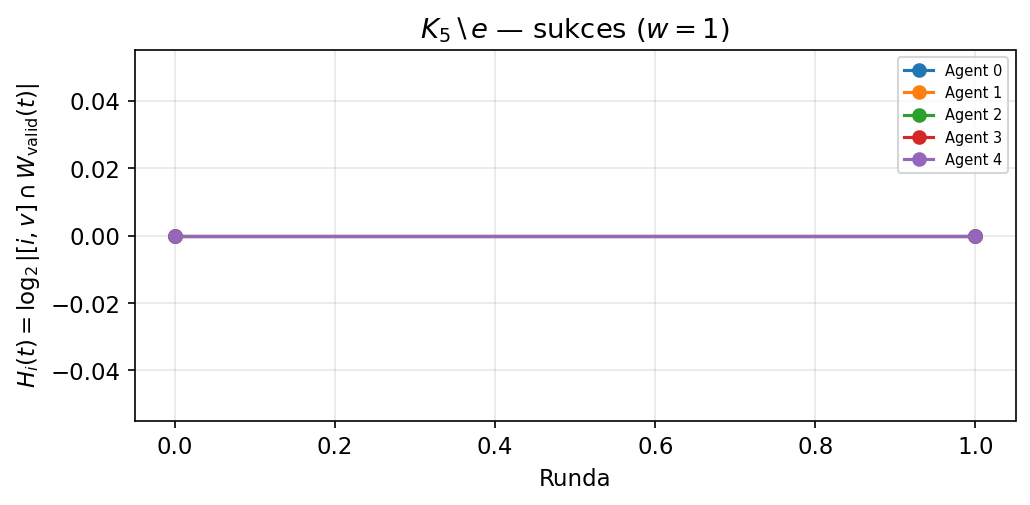
\includegraphics[width=\linewidth]{fig_entropy_k5e_k3.png}
    \caption{Sukces: $w=00111_2$\\ ($k=3$, węzły 0,1,2)}
  \end{subfigure}
  \hfill
  \begin{subfigure}[t]{0.30\textwidth}
    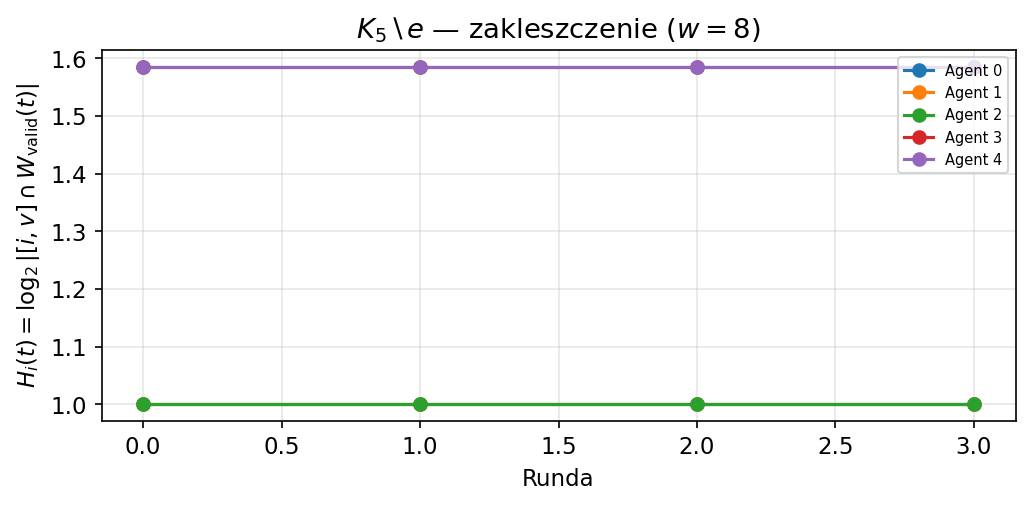
\includegraphics[width=\linewidth]{fig_entropy_k5e_dead.png}
    \caption{Zakleszczenie: $w=01000_2$\\ (węzeł 3 sam czerwony)}
  \end{subfigure}
  \caption{$K_5 \setminus \{3,4\}$: struktura grafu i kontrastujące ślady entropii.
    Agenci 0--2 (stopień 4) odgadują kaskadowo; agenci 3, 4 (stopień 3) kleszczą gdy jeden z nich jest czerwony.}
  \label{fig:kne}
\end{figure}

\begin{theorem}
\label{thm:kne}
Dla $K_n \setminus \{u,v\}$ i każdego $w \ge 1$:
$$\rounds(K_n \setminus \{u,v\},\, w) < \infty \;\iff\; \mathrm{bit}_u(w) = 0 \;\wedge\; \mathrm{bit}_v(w) = 0.$$
W przypadku sukcesu $\rounds = \min(k, n-3)$, gdzie $k = \popcount(w)$.
\end{theorem}

Pełny dowód podano w sekcji~\ref{sec:proof_kne}.

% ─────────────────────────────────────────────────────────────────────────────
\subsection{Przegląd porównawczy topologii}

\begin{figure}[H]
  \centering
  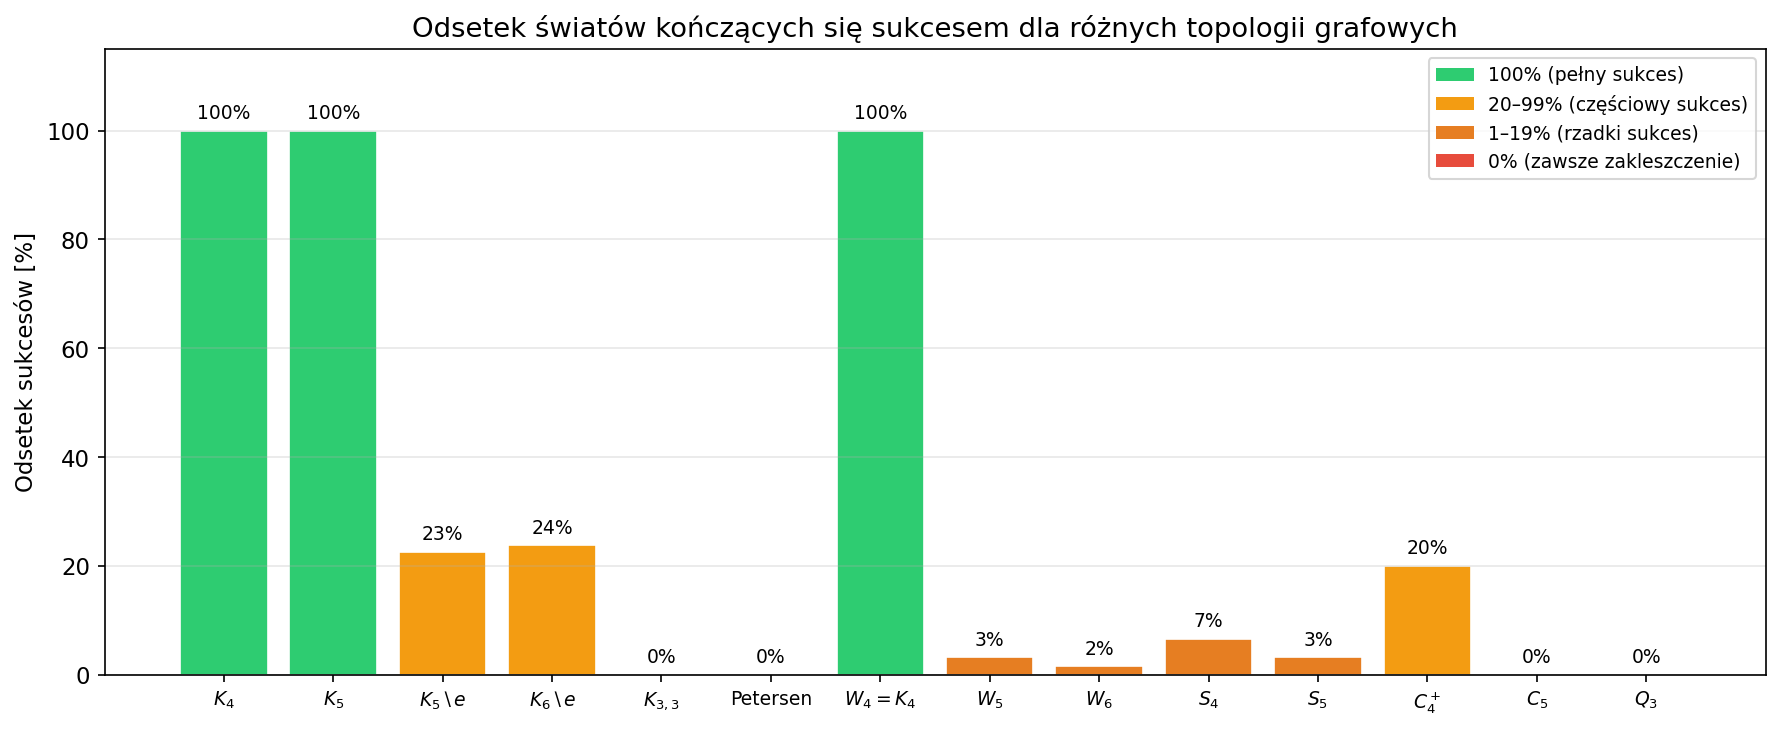
\includegraphics[width=\textwidth]{fig_success_rates.png}
  \caption{Odsetek światów kończących się sukcesem dla różnych topologii grafowych.
    Wyraźny podział: $K_n$ (100\%), $K_n\setminus e$ (ok.\ 24\%), topologie specjalne ($\le 4\%$), struktury symetryczne i bipartite (0\%) — w tym $K_{3,3}$ i graf Petersena.}
  \label{fig:rates}
\end{figure}

% ─────────────────────────────────────────────────────────────────────────────
\subsection{Graf dwudzielny $K_{m,n}$ i Zagadka Trzech Mediów}
\label{sec:bipartite}

\textbf{Definicja.} Graf dwudzielny $K_{m,n}$ ma dwie rozłączne grupy wierzchołków $A = \{0,\ldots,m{-}1\}$ i $B = \{m,\ldots,m{+}n{-}1\}$; krawędzie łączą każdy wierzchołek z $A$ z każdym z $B$, lecz brak krawędzi wewnątrz grup:
$$\deg(u) = n \;\text{ dla } u \in A, \qquad \deg(v) = m \;\text{ dla } v \in B.$$

\textbf{Zagadka Trzech Mediów ($K_{3,3}$).} Klasyczna łamigłówka kombinatoryczna pyta, czy można poprowadzić przewody od każdego z 3 domów do każdego z 3 mediów (woda, gaz, prąd) bez wzajemnych przecięć. Graf $K_{3,3}$ jest matematyczną istotą tej zagadki — odpowiedź brzmi \emph{nie}, gdyż $K_{3,3}$ nie jest planarny. Polskim akcentem jest \textbf{twierdzenie Kuratowskiego} (1930): graf jest planarny wtedy i tylko wtedy, gdy nie zawiera topologicznego podziału $K_5$ ani $K_{3,3}$.

\begin{figure}[H]
  \centering
  \begin{subfigure}[t]{0.42\textwidth}
    \centering
    \begin{tikzpicture}[scale=0.85,
        every node/.style={circle,draw,minimum size=0.72cm,font=\small\bfseries}]
      \node[fill=blue!20]  (3) at (0, 2.0) {3};
      \node[fill=blue!20]  (4) at (2, 2.0) {4};
      \node[fill=blue!20]  (5) at (4, 2.0) {5};
      \node[fill=green!25] (0) at (0, 0)   {0};
      \node[fill=green!25] (1) at (2, 0)   {1};
      \node[fill=green!25] (2) at (4, 0)   {2};
      \foreach \u in {0,1,2}
        \foreach \v in {3,4,5}
          \draw[thick] (\u) -- (\v);
      \node[draw=none,fill=none,font=\small] at (-1.0, 2.0) {$B$};
      \node[draw=none,fill=none,font=\small] at (-1.0, 0.0) {$A$};
    \end{tikzpicture}
    \caption{Graf $K_{3,3}$: partycja $A$ (zielona) i $B$ (niebieska). Brak krawędzi wewnątrz grup.}
  \end{subfigure}
  \hfill
  \begin{subfigure}[t]{0.55\textwidth}
    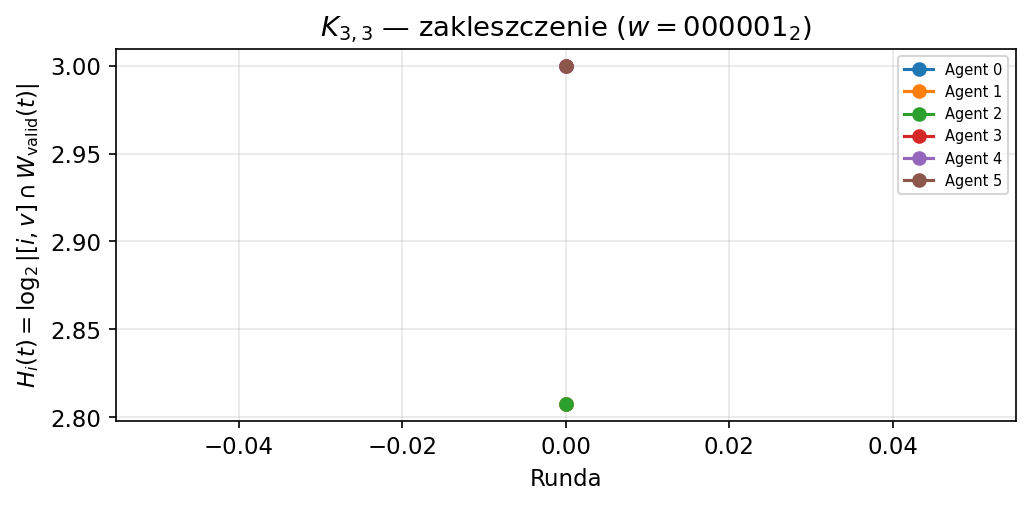
\includegraphics[width=\linewidth]{fig_entropy_k33_dead.png}
    \caption{Entropia epistemiczna $K_{3,3}$, $w=1$ — punkt stały dla wszystkich 6 agentów.}
  \end{subfigure}
  \caption{$K_{3,3}$: graf Zagadki Trzech Mediów i jego entropia epistemiczna (zawsze zakleszczenie).}
\end{figure}

\begin{table}[H]
\centering
\caption{Graf dwudzielny $K_{m,n}$ — wyniki symulacji wyczerpujące}
\begin{tabular}{ccccc}
\toprule
Graf & Wierzchołki & Sukces & Razem & Wynik \\
\midrule
$K_{2,2} = C_4$ & 4 & 0 & 15  & Zakleszczenie \\
$K_{2,3}$       & 5 & 0 & 31  & Zakleszczenie \\
$K_{3,3}$       & 6 & 0 & 63  & Zakleszczenie \\
$K_{2,4}$       & 6 & 0 & 63  & Zakleszczenie \\
$K_{3,4}$       & 7 & 0 & 127 & Zakleszczenie \\
\bottomrule
\end{tabular}
\end{table}

\begin{theorem}
\label{thm:bipartite}
Dla $K_{m,n}$ z $m,n \ge 2$ i każdego $w \ge 1$: $\rounds(K_{m,n}, w) = \infty$.
\end{theorem}

\begin{proof}[Zarys dowodu]
Wierzchołek $u \in A$ widzi $n$ sąsiadów z $B$ i nie widzi $m-1$ wierzchołków z $A$. Jego klasa $[u, \view_u(w)]$ ma $m \ge 2$ wolne bity (własny bit $u$ oraz bity $A \setminus \{u\}$), skąd $2^m \ge 4$ światów z oboma kolorami bitu $u$ — niejednorodna. Symetrycznie każdy $v \in B$ ma $n \ge 2$ wolne bity. Żadna klasa nie jest jednorodna $\Rightarrow$ zakleszczenie. $\square$
\end{proof}

\begin{remark}
$K_{1,n} = S_n$ (gwiazda, $m=1$) jest wyjątkiem: centrum ma $\deg = n-1$ i 1 wolny bit, co pozwala mu odgadnąć w szczególnym przypadku $w=1$ (twierdzenie~\ref{thm:star}).
\end{remark}

% ─────────────────────────────────────────────────────────────────────────────
\subsection{Graf Petersena — król kontrprzykładów}
\label{sec:petersen}

Graf Petersena to 3-regularny, 10-wierzchołkowy graf sławny jako \emph{kontrprzykład} dla wielu twierdzeń teorii grafów: nie jest Hamiltonowski, ma indeks chromatyczny 4, a mimo to posiada wysoką symetrię (tranzytywność na krawędziach). Konstruujemy go jako:
\begin{itemize}
  \item zewnętrzny pięciokąt: $0$--$1$--$2$--$3$--$4$--$0$,
  \item wewnętrzna pięciogwiazda: $5$--$7$--$9$--$6$--$8$--$5$,
  \item szprychy: $\{0,5\},\{1,6\},\{2,7\},\{3,8\},\{4,9\}$.
\end{itemize}

\begin{figure}[H]
  \centering
  \begin{subfigure}[t]{0.38\textwidth}
    \centering
    \begin{tikzpicture}[scale=1.05,
        every node/.style={circle,draw,minimum size=0.68cm,font=\small\bfseries}]
      \foreach \i/\angle in {0/90, 1/162, 2/234, 3/306, 4/18}
        \node (\i) at (\angle:2.0) {\i};
      \foreach \i/\angle in {5/90, 6/162, 7/234, 8/306, 9/18}
        \node[fill=gray!20] (\i) at (\angle:1.05) {\i};
      \foreach \a/\b in {0/1, 1/2, 2/3, 3/4, 4/0}
        \draw[thick] (\a) -- (\b);
      \foreach \a/\b in {5/7, 7/9, 9/6, 6/8, 8/5}
        \draw[thick] (\a) -- (\b);
      \foreach \a/\b in {0/5, 1/6, 2/7, 3/8, 4/9}
        \draw[thick] (\a) -- (\b);
    \end{tikzpicture}
    \caption{Graf Petersena (10 wierzchołków, stopień 3).}
  \end{subfigure}
  \hfill
  \begin{subfigure}[t]{0.59\textwidth}
    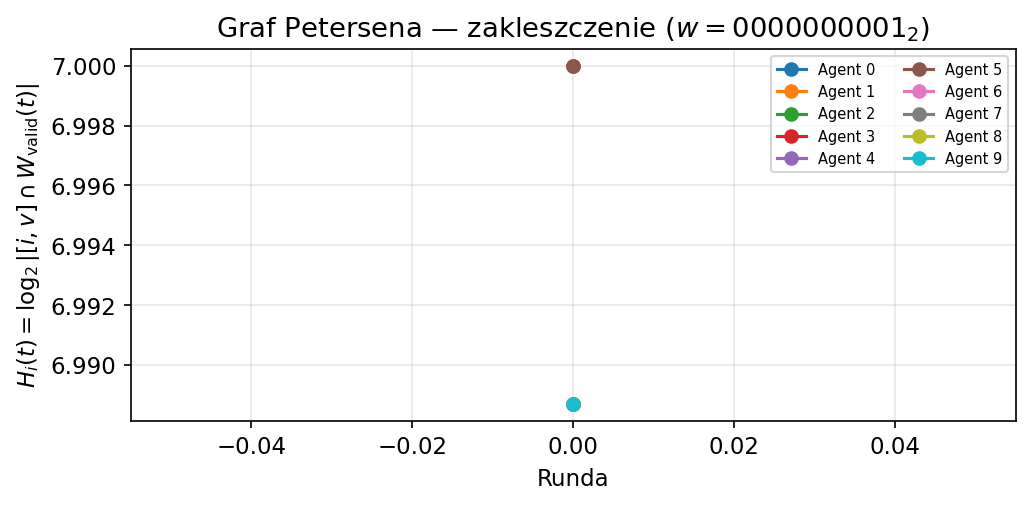
\includegraphics[width=\linewidth]{fig_entropy_petersen_dead.png}
    \caption{Entropia epistemiczna — zakleszczenie dla $w=1$. Wszystkie 10 agentów w punkcie stałym.}
  \end{subfigure}
  \caption{Graf Petersena: estetyczna symetria grafowa okazuje się przeszkodą epistemiczną.}
\end{figure}

\begin{table}[H]
\centering
\caption{Graf Petersena — wyczerpująca analiza 1023 światów}
\begin{tabular}{lc}
\toprule
Miara & Wartość \\
\midrule
Wierzchołki & 10 \\
Stopień każdego wierzchołka & 3 \\
Wolne bity na agenta & $10 - 3 - 1 = 6$ \\
Zakleszczenia & 1023 / 1023 \\
Sukcesy & 0 / 1023 \\
\bottomrule
\end{tabular}
\end{table}

\textbf{Wyjaśnienie.} Każdy wierzchołek ma $10 - 3 - 1 = 6$ wolnych bitów, co daje $2^6 = 64$ światów w każdej klasie z oboma kolorami własnego bitu. Wysoka symetria grafu gwarantuje brak żadnej klasy jednorodnej — identyczny efekt jak w $C_n$ i $Q_k$. Graf Petersena, choć jest ``królem kontrprzykładów'' teorii grafów, sam staje się kontrprzykładem hipotezy: ,,bogata łączność gwarantuje sukces epistemiczny.''

% ─────────────────────────────────────────────────────────────────────────────
\subsection{Grafy bezskalowe i sieci rzeczywiste}
\label{sec:scalefree}

\textbf{Model Barabásiego–Alberta.} Grafy bezskalowe generowane modelem preferencyjnego dołączania (Barabási, Albert, 1999) opisują strukturę Internetu, sieci społecznościowych i połączeń lotniczych. Cechuje je rozkład stopni $P(k) \sim k^{-\gamma}$ ($\gamma \approx 2{,}5$): nieliczne węzły (\emph{huby}) mają stopień rzędu setek, natomiast większość węzłów ma stopień 1--3.

\textbf{Implikacje dla gry epistemicznej.} Z udowodnionych twierdzeń wynika bezpośrednia konsekwencja:
\begin{enumerate}
  \item Każdy węzeł o $\deg(i) < n-1$ posiada co najmniej 1 wolny bit $\Rightarrow$ własny bit leży w obu kolorach klasy $\Rightarrow$ agent nie może samodzielnie odgadnąć.
  \item Warunek konieczny sukcesu: \emph{każdy} agent musi \emph{ostatecznie} uzyskać jednorodną klasę. Z dowodu twierdzenia~\ref{thm:kn} wynika, że wymaga to $\deg(i) = n-1$ lub kaskadowej eliminacji przez wcześniejszych zgadujących.
  \item W grafie bezskalowym węzły o małym stopniu ($\deg = O(1) \ll n$) mają klasy z $2^{n-O(1)}$ światami — nie ma szans na jednorodność bez dodatkowych ogłoszeń. Skoro sami nie mogą odgadnąć, nie inicjują kaskady.
\end{enumerate}

\textbf{Analogia ze $S_n$.} $S_n$ jest ekstremalną instancją sieci bezskalowej: jeden hub ($\deg = n-1$) i $n-1$ liści ($\deg = 1$). Twierdzenie~\ref{thm:star} dowiodło zakleszczenia dla prawie wszystkich konfiguracji — jedyny wyjątek $w=1$ jest możliwy wyłącznie dlatego, że hub widzi \emph{wszystkich} liści naraz. W realistycznych grafach bezskalowych nawet huby mają $\deg \ll n$, co eliminuje ten wyjątek.

\begin{corollary}[Kryterium gęstości]
\label{cor:density}
Niech $G$ będzie grafem na $n$ wierzchołkach. Warunkiem koniecznym (choć niewystarczającym) rozwiązywalności gry na $(G, w)$ jest istnienie agenta $i$ z $\deg(i) = n-1$ (połączonego ze wszystkimi pozostałymi) \textbf{lub} kaskadowej struktury, w której pierwotna jednorodność pewnego agenta inicjuje eliminację prowadzącą do jednorodności pozostałych.

W szczególności: $K_{m,n}$ ($m,n \ge 2$), graf Petersena, $C_n$ ($n \ge 4$), $Q_k$ ($k \ge 2$) i typowe grafy bezskalowe nie spełniają żadnego z tych warunków — zawsze kleszczą.
\end{corollary}

% ─────────────────────────────────────────────────────────────────────────────
\subsection{Graf uporządkowanej widoczności $O_n$}
\label{sec:ordered}

\textbf{Definicja.} W grafie $O_n$ ($n \ge 2$) wierzchołki są ustawione w liniowym porządku $0, 1, \ldots, n{-}1$. Relacja widoczności jest \emph{skierowana i zhierarchizowana}: wierzchołek $k$ widzi wyłącznie wierzchołki o wyższym indeksie:
$$N(k) = \{k+1,\, k+2,\, \ldots,\, n-1\}.$$
W szczególności: $\deg(0) = n-1$ (widzi wszystkich), $\deg(n-1) = 0$ (nie widzi nikogo).

\begin{figure}[H]
  \centering
  \begin{tikzpicture}[scale=1.0, >=Stealth,
      every node/.style={circle,draw,minimum size=0.72cm,font=\small\bfseries}]
    \foreach \i in {0,...,4}
      \node (\i) at (\i*2, 0) {\i};
    % Directed edges: k -> j for k < j; show only direct forward edges to keep it readable
    \foreach \a/\b in {0/1, 1/2, 2/3, 3/4}
      \draw[->,thick] (\a) -- (\b);
    % Long-range edges for vertex 0
    \draw[->,thick,bend left=30] (0) to (2);
    \draw[->,thick,bend left=35] (0) to (3);
    \draw[->,thick,bend left=40] (0) to (4);
    % Long-range for vertex 1
    \draw[->,thick,bend right=25] (1) to (3);
    \draw[->,thick,bend right=30] (1) to (4);
    % Long-range for vertex 2
    \draw[->,thick,bend left=20] (2) to (4);
    % label
    \node[draw=none,fill=none,font=\small] at (4, -1.2) {(tylko strzałki w prawo)};
  \end{tikzpicture}
  \caption{Graf uporządkowanej widoczności $O_5$: wierzchołek $k$ widzi wyłącznie $\{k{+}1,\ldots,4\}$. Relacja widoczności jest asymetryczna (skierowana).}
  \label{fig:o5}
\end{figure}

\begin{table}[H]
\centering
\caption{Graf $O_n$ — wyniki wyczerpujące}
\begin{tabular}{cccc}
\toprule
$n$ & Sukces & Razem & Jedyny świat sukcesu \\
\midrule
2  & 1 & 3    & $w = 01_2$ (tylko wierzchołek 0) \\
3  & 1 & 7    & $w = 001_2$ \\
4  & 1 & 15   & $w = 0001_2$ \\
5  & 1 & 31   & $w = 00001_2$ \\
6  & 1 & 63   & $w = 000001_2$ \\
7  & 1 & 127  & $w = 0000001_2$ \\
8  & 1 & 255  & $w = 00000001_2$ \\
10 & 1 & 1023 & $w = 0000000001_2$ \\
\bottomrule
\end{tabular}
\end{table}

\begin{figure}[H]
  \centering
  \begin{subfigure}[t]{0.48\textwidth}
    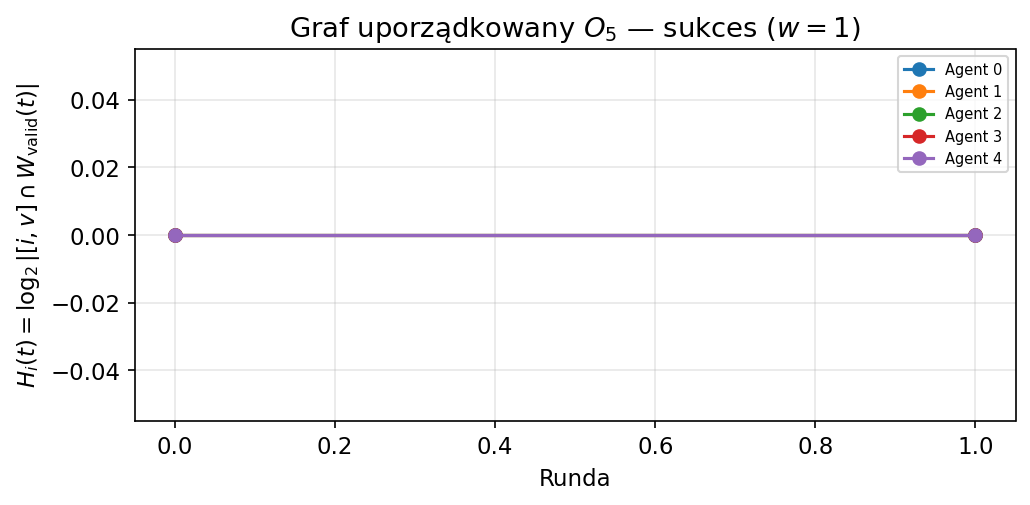
\includegraphics[width=\linewidth]{fig_entropy_o5_succ.png}
    \caption{Sukces: $w=00001_2$ (tylko wierzchołek 0 czerwony).}
  \end{subfigure}
  \hfill
  \begin{subfigure}[t]{0.48\textwidth}
    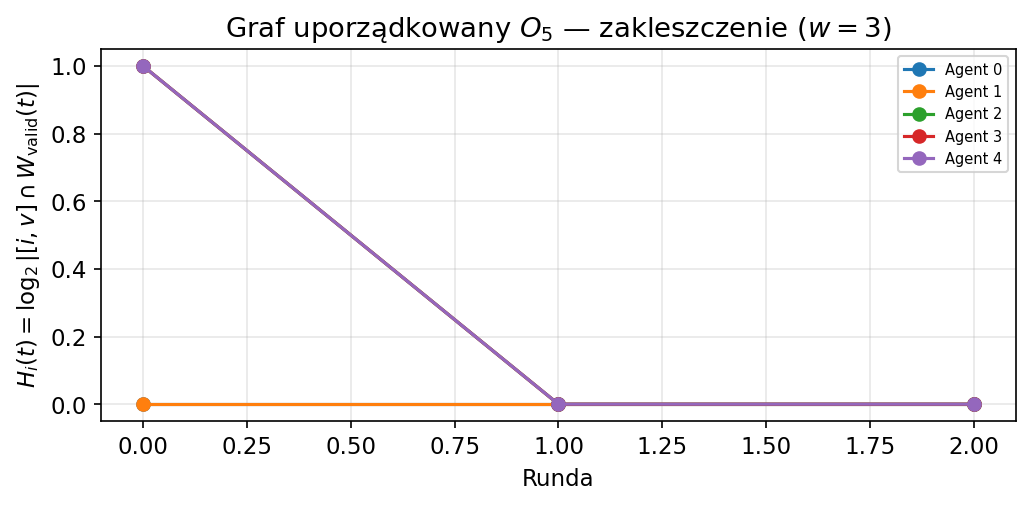
\includegraphics[width=\linewidth]{fig_entropy_o5_dead.png}
    \caption{Zakleszczenie: $w=00011_2$ (wierzchołki 0 i 1 czerwone).}
  \end{subfigure}
  \caption{$O_5$: entropia epistemiczna dla jedynego sukcesu i reprezentatywnego zakleszczenia. W sukcesie: ogłoszenie agenta 0 natychmiast redukuje $|\Wval| \to 1$; wszyscy pozostali odgadują w rundzie~1.}
\end{figure}

\begin{theorem}
\label{thm:ordered}
Dla grafu $O_n$ ($n \ge 2$) jedynym światem prowadzącym do sukcesu jest $w = 1$ (tylko wierzchołek 0 nosi czerwony kapelusz). Dla wszystkich pozostałych $w \in \{2, \ldots, 2^n{-}1\}$: $\rounds(O_n, w) = \infty$.

W przypadku sukcesu $\rounds(O_n, 1) = 1$ (dwa zdarzenia: wierzchołek 0 odgaduje, następnie wszyscy pozostali).
\end{theorem}

\begin{proof}
\textbf{Sukces dla $w = 1$:} Wierzchołek 0 widzi $\{1,\ldots,n{-}1\}$; $\view_0(1) = 0$ (wszyscy biali). Klasa $[0,0] \cap \Wval = \{1\}$ — singleton (świat 0 wykluczony). Agent 0 odgaduje czerwony.

Ogłoszenie publiczne: \emph{,,agent 0 jest czerwony I wiedział to.''} Eliminuje to dwie grupy światów: (1) $\{w': \mathrm{bit}_0(w') = 0\}$ (zły kolor) oraz (2) $\{w': \text{klasa agenta 0 niejednorodna}\}$ (agent nie mógłby zgadnąć). Klasa agenta 0 jest singletonem jedynie w świecie~1; we wszystkich innych $w' \ne 1$ z $\mathrm{bit}_0 = 1$ klasa = $\{w', w'+1\}$ (dwuelementowa). Zatem po ogłoszeniu $\Wval = \{1\}$.

Każdy $i \ge 1$: klasa $\cap \{1\} = \{1\}$ — singleton. Odgaduje biały ($\mathrm{bit}_i(1) = 0$). $\rounds = 1$.

\textbf{Zakleszczenie dla $w \ne 1$:} Kluczowa obserwacja: dla dowolnego $w' \ne 0, 1$, $w' \ne 1$ implikuje $w'$ i $w' \oplus 1 = w' \pm 1$ mają te same bity $1, \ldots, n{-}1$ (flipa tylko bit 0). Zatem:
\begin{enumerate}
  \item Agent 0's view $\view_0(w') = w' \& (2^n{-}2)$ jest taki sam dla $w'$ i $w' \oplus 1$.
  \item Agent $k$ ($k \ge 1$) widzi bity $k{+}1, \ldots, n{-}1$: jego widok też nie różnicuje $w'$ i $w' \oplus 1$.
\end{enumerate}
Światy $w$ i $w \oplus 1$ są \emph{nierozróżnialne} przez wszystkich agentów — zarówno pod kątem ciszy (eliminacja zbiorowa), jak i odgadywań. Agent 0 może wyeliminować $w \oplus 1$ jedynie własnym odgadnięciem bitu 0, ale agent 0 może odgadnąć tylko gdy klasa jest singletonem, co wymaga $w \oplus 1 \notin \Wval$ — warunek kołowy.

Stąd światy $\{w, w \oplus 1\}$ (para bitowa na bicie 0) zawsze pozostają razem w $\Wval$. Ich klasy są zawsze niejednorodne. Żaden agent nie może odgadnąć. Zakleszczenie. $\square$
\end{proof}

\begin{remark}[Związek z klasyczną zagadką kapeluszy]
Wariant $O_n$ odpowiada \emph{klasycznej zagadce kapeluszy w porządku liniowym} (Berlekamp, 1964; Winkler, 2002): agenci widzą kapelusze wszystkich stojących przed nimi, lecz zgadują jednocześnie bez komunikacji. W klasycznym wariancie (bez publicznych oznajmień) strategia oparta na arytmetyce modularnej gwarantuje co najmniej jedno poprawne odgadnięcie. W naszym wariancie iteracyjnym (DEL, wymagającym bezbłędności \emph{wszystkich}) wynik jest drastycznie silniejszy: tylko $w = 1$ kończy się pełnym sukcesem — jedna pomyłka ($w \ne 1$) prowadzi do zakleszczenia.
\end{remark}

% ─────────────────────────────────────────────────────────────────────────────
\section{Dowody matematyczne}

\subsection{Graf pełny $K_n$: $\rounds(K_n,w) = \min(k, n-1)$}
\label{sec:proof_kn}

\begin{theorem}
\label{thm:kn}
Dla grafu pełnego $K_n$ i każdego $w \in \{1,\ldots,2^n{-}1\}$ z $k = \popcount(w)$:
$$\rounds(K_n, w) = \min(k,\, n-1).$$
W szczególności gra zawsze kończy się sukcesem.
\end{theorem}

\begin{lemma}[Klasy partycji w $K_n$]
\label{lem:kn_classes}
W $K_n$ agent $i$ widzi wszystkich $n{-}1$ pozostałych agentów: $N(i) = V \setminus \{i\}$. Klasa $[i,v]$ zawiera dokładnie dwa światy: $v$ (bit $i = 0$) i $v + 2^i$ (bit $i = 1$).
\end{lemma}

\begin{proof}
Dwa światy $w, w'$ spełniają $w \sim_i w'$ iff $w \;\&\; (2^n{-}1{-}2^i) = w' \;\&\; (2^n{-}1{-}2^i)$, tzn.\ zgadzają się na wszystkich bitach poza $i$. Jedyną swobodą jest bit $i$. $\square$
\end{proof}

\begin{lemma}[Dynamika rund ciszy]
\label{lem:kn_silence}
Niech $\Wval_j$ będzie zbiorem ważnych światów po $j$ rundach ciszy. Wtedy:
$$\Wval_j = \{w \in \{1,\ldots,2^n{-}1\} : \popcount(w) > j\}.$$
\end{lemma}

\begin{proof}
\textbf{Baza} ($j=0$): $\Wval_0 = \{1,\ldots,2^n{-}1\}$ to dokładnie światy z $\popcount(w) \ge 1 > 0$. ✓

\textbf{Krok indukcyjny}: Zakładamy $\Wval_j = \{w : \popcount(w) > j\}$. Runda ciszy eliminuje świat $w' \in \Wval_j$, gdy klasa $[i, \view_i(w')] \cap \Wval_j$ jest jednorodna dla pewnego agenta $i$. Z lematu~\ref{lem:kn_classes} klasa = $\{v,\, v{+}2^i\} \cap \Wval_j$. Ta para jest jednorodna (singleton) iff jeden z elementów $\notin \Wval_j$. Element $v = w' \;\&\; (2^n{-}1{-}2^i)$ (bit $i = 0$) ma $\popcount(v) = \popcount(w') - \mathrm{bit}_i(w')$. Jeśli $\mathrm{bit}_i(w') = 1$: $\popcount(v) = \popcount(w') - 1$. Singleton iff $v \notin \Wval_j$, tzn.\ $\popcount(v) \le j$, tzn.\ $\popcount(w') - 1 \le j$, tzn.\ $\popcount(w') = j+1$. Eliminowane są zatem dokładnie światy z $\popcount = j+1$:
$$\Wval_{j+1} = \Wval_j \setminus \{w : \popcount(w) = j+1\} = \{w : \popcount(w) > j+1\}. \quad \square$$
\end{proof}

\begin{proof}[Dowód twierdzenia~\ref{thm:kn}]
\textbf{Przypadek $k \le n-1$:} Po $k-1$ rundach ciszy $\Wval_{k-1} = \{w : \popcount(w) \ge k\}$. Agent $i$ z $\mathrm{bit}_i(w) = 1$ (kapelusz czerwony) widzi $k-1$ sąsiadów czerwonych: $\view_i(w) = v$ z $\popcount(v) = k-1$. Klasa $[i,v] \cap \Wval_{k-1} = \{v, v+2^i\} \cap \Wval_{k-1}$. Ponieważ $\popcount(v) = k-1 \le k-1$, mamy $v \notin \Wval_{k-1}$, czyli klasa = $\{v+2^i\}$ — jednorodna. Agent odgaduje czerwony w zdarzeniu numer $k$. Po tym odgadnięciu agenci z białymi kapeluszami (widzący $k$ czerwonych) mają klasę $\{w\}$ — odgadują białe w kolejnym zdarzeniu terminalnym (bez inkrementacji licznika). Łącznie: $k{-}1$ rund ciszy $+$ 1 eliminacja $= k$ zdarzeń, czyli $\rounds = k$.

\textbf{Przypadek $k = n$:} Po $n-1$ rundach ciszy $\Wval_{n-1} = \{w : \popcount(w) \ge n\} = \{2^n{-}1\}$. Wszyscy agenci jednocześnie odgadują czerwony — zdarzenie terminalne bez inkrementacji licznika. $\rounds = n-1$.

Łącząc oba przypadki: $\rounds(K_n,w) = \min(k, n-1)$. $\square$
\end{proof}

\begin{remark}[Konwencja licznika rund]
Przypadek $k = n$ wymaga osobnej analizy: klasyczna Zagadka Zabrudzonych Dzieci (Fagin et al., 1995) zlicza $k$ deklaracji łącznie z ostateczną odpowiedzią, natomiast nasz licznik rejestruje wyłącznie zdarzenia z \emph{eliminacją} stanu przestrzeni. Ostateczne jednoczesne odgadnięcie (zdarzenie terminalne) nie powoduje inkrementacji — stąd $\rounds = n{-}1$, a nie $n$. Formuła $\min(k,n-1)$ jest potwierdzona empirycznie dla $n = 3,\ldots,14$ przy wszystkich wartościach $k$ oraz dla $k=1$ przy $n \le 24$.
\end{remark}

\subsection{Cykl $C_n$ dla $n \ge 4$: niezmiennik zakleszczenia}
\label{sec:proof_cn}

\begin{theorem}
\label{thm:cn}
Dla cyklu $C_n$ z $n \ge 4$ i każdego $w \in \{1,\ldots,2^n{-}1\}$: $\rounds(C_n,w) = \infty$.
\end{theorem}

\begin{lemma}[Niejednorodność klas w $C_n$]
\label{lem:cn_classes}
W $C_n$ ($n \ge 4$) dla każdego agenta $i$, każdej obserwacji $v$ i każdego $\Wval \supseteq \{w : \popcount(w) = p\}$ (dla $p \ge 1$), klasa $[i,v] \cap \Wval$ jest niejednorodna (zawiera oba kolory bitu $i$).
\end{lemma}

\begin{proof}
Agent $i$ widzi sąsiadów $i_- = (i-1) \bmod n$ i $i_+ = (i+1) \bmod n$. Klasa $[i,v]$ określona jest przez $\mathrm{bit}_{i_-}$ i $\mathrm{bit}_{i_+}$; pozostałe $n-2$ bitów (w tym bit $i$ i $n-3$ innych) są wolne. Ponieważ $n \ge 4$, mamy $n-2 \ge 2$. Niech $j \in V \setminus \{i,i_-,i_+\}$ (taki $j$ istnieje, bo $n-3 \ge 1$ dla $n \ge 4$). Klasa zawiera co najmniej cztery światy:
$$w_0 = v,\quad w_1 = v+2^i,\quad w_2 = v+2^j,\quad w_3 = v+2^i+2^j.$$
Ponieważ $j \notin \{i_-,i_+\}$, dodanie $2^j$ nie zmienia wartości $v = w \;\&\; \mask_i$. Wszystkie cztery światy leżą w $[i,v]$. Spośród nich $w_0, w_2$ mają $\mathrm{bit}_i = 0$, a $w_1, w_3$ mają $\mathrm{bit}_i = 1$. Conajmniej jeden z nich $\ne 0$ (bo $v \ne 0$ lub $2^i+2^j \ne 0$), więc klasa ma $\ge 2$ światów ważnych z oboma kolorami. $\square$
\end{proof}

\begin{proof}[Dowód twierdzenia~\ref{thm:cn}]
Z lematu~\ref{lem:cn_classes} wynika, że $[i,v] \cap \Wval_0$ jest niejednorodna dla każdego $(i,v)$.

Żaden agent nie może odgadnąć w rundzie~0. Runda ciszy eliminuje tylko światy $w'$, dla których istnieje $(i,v)$ z jednorodną klasą $[i,v]\cap\Wval_0$. Skoro żadna klasa nie jest jednorodna, $\Wval_1 = \Wval_0$. Przez indukcję $\Wval_t = \Wval_0$ dla wszystkich $t$. Brak eliminacji przez \texttt{apply\_silence} skutkuje zakleszczeniem. $\square$
\end{proof}

\begin{remark}
$C_3 = K_3$ jest wyjątkiem: dla $n = 3$ agent $i$ widzi $n-1 = 2$ sąsiadów, co daje stopień $n-2=1$ wolny bit (wyłącznie własny bit $i$). Klasa ma co najwyżej 2 światy, a wykluczenie $\Wval_0 \not\ni 0$ powoduje, że klasa dla widoku ``obie biali'' jest singletonem $\{2^i\}$. $C_3$ zachowuje się jak $K_3$.
\end{remark}

\subsection{Graf gwiazdowy $S_n$: jedyna rozwiązywalna konfiguracja}

\begin{theorem}
\label{thm:star}
Dla $S_n$ ($n \ge 2$, centrum = agent 0):
$$\rounds(S_n,w) < \infty \;\iff\; w = 1 \;\text{(samo centrum czerwone).}$$
W przypadku sukcesu $\rounds(S_n,1) = 1$.
\end{theorem}

\begin{proof}
\textbf{Sukces dla $w = 1$:} Centrum widzi wszystkie liście białe: $\view_0(1) = 1 \;\&\; \mask_0 = 0$. Klasa $[0,0] = \{0,1\} \cap \Wval_0 = \{1\}$ — singleton. Centrum odgaduje czerwony. Po ogłoszeniu wszystkie światy poza $\{1\}$ są eliminowane; każdy liść $i$ ma klasę $[i,1] \cap \{1\} = \{1\}$ z $\mathrm{bit}_i(1) = 0$ — odgadują białe. $\rounds = 1$.

\textbf{Zakleszczenie dla $w \ne 1$:}

\emph{Przypadek A: centrum białe} ($\mathrm{bit}_0(w) = 0$, $w \ne 0$). Każdy liść $i$ widzi centrum białe: $\view_i(w) = 0$. Klasa liścia $i$ dla widoku 0 zawiera wszystkie światy z $\mathrm{bit}_0 = 0$, wśród których $\mathrm{bit}_i$ przybiera obie wartości (liść $i$ czerwony lub biały). Klasa niejednorodna. Centrum widzi liście i ma klasę $\{v_0, v_0 + 1\}$ z $v_0 = w\;\&\;\mask_0 \ne 0$ (bo $w \ne 0$) i $v_0$ parzystym. Oba światy są ważne ($v_0 \ge 2$), klasa niejednorodna. Żadna klasa nie jest jednorodna $\Rightarrow$ zakleszczenie.

\emph{Przypadek B: centrum czerwone, co najmniej jeden liść czerwony}. Każdy liść $i$ widzi centrum czerwone: $\view_i(w) = 1$. Klasa $[i,1]$ zawiera wszystkie $2^{n-1}$ światów z $\mathrm{bit}_0 = 1$; $\mathrm{bit}_i$ wolny $\Rightarrow$ niejednorodna. Centrum widzi co najmniej jeden liść czerwony: $v_0 = w\;\&\;\mask_0 \ne 0$. Klasa centrum = $\{v_0, v_0+1\}$, oba $\ge 2 \Rightarrow$ oba ważne $\Rightarrow$ niejednorodna. Żadna klasa nie jest jednorodna $\Rightarrow$ zakleszczenie. $\square$
\end{proof}

\begin{remark}
Liść widzi wyłącznie centrum, a jego klasa zawiera zawsze oba kolory własnego bitu niezależnie od koloru centrum — liście \emph{nigdy} nie mogą samodzielnie odgadnąć swojego koloru bez wcześniejszego odgadnięcia centrum. Jedyną rozwiązywalną konfiguracją na dowolnym $S_n$ jest $w = 1$.
\end{remark}

\subsection{Graf ścieżkowy $P_n$ dla $n \ge 4$: zawsze zakleszczenie}

\begin{theorem}
\label{thm:path}
Dla $P_n$ z $n \ge 4$ i każdego $w \ge 1$: $\rounds(P_n,w) = \infty$.
\end{theorem}

\begin{proof}
W $P_n$ agent $i$ wewnętrzny ($0 < i < n{-}1$) widzi $\{i{-}1, i{+}1\}$. Jego klasa $[i,v]$ ma wolne bity: bit $i$ (własny) oraz bity $j \notin \{i{-}1,i,i{+}1\}$ (nie-sąsiedzi różni od siebie). Dla $n \ge 4$ istnieje co najmniej jeden taki $j$ ($n \ge 4 \Rightarrow n-3 \ge 1$), więc klasa ma $\ge 4$ światów z oboma kolorami bitu $i$ — niejednorodna.

Agenci końcowi ($i = 0$ lub $i = n{-}1$) widzą jednego sąsiada; ich klasy mają $2^{n-2}$ weltów z wolnymi $n-2 \ge 2$ bitami (własnym i $n-3$ nie-sąsiadów) — niejednorodne.

Żadna klasa nie jest jednorodna $\Rightarrow$ zakleszczenie. $\square$
\end{proof}

\begin{corollary}
$P_n$ dla $n \ge 4$ jest izomorficzne pod względem dynamiki gry z $C_n$ dla $n \ge 4$: oba zawsze kleszczą. Natomiast $P_3 \cong S_3 \cong K_{1,2}$ posiada jedną rozwiązywalną konfigurację ($w = 2$, środkowy wierzchołek czerwony).
\end{corollary}

\subsection{Hiperkostka $Q_k$ dla $k \ge 2$: zawsze zakleszczenie}
\label{sec:hypercube}

\begin{theorem}
\label{thm:hypercube}
Hiperkostka $Q_k$ dla $k \ge 2$ i każdego $w \ge 1$: $\rounds(Q_k,w) = \infty$.
\end{theorem}

\begin{proof}
W $Q_k$ każdy węzeł $i$ ma stopień $k$ (sąsiedzi to $i \oplus 2^p$ dla $p = 0,\ldots,k{-}1$). Klasa $[i,v]$ w $Q_k$ o $n = 2^k$ węzłach ma wolnych $n - k - 1 = 2^k - k - 1$ bitów (nie-sąsiedzi różni od siebie). Dla $k \ge 2$: $2^k - k - 1 \ge 4 - 2 - 1 = 1$, a w szczególności bit $i$ jest wolny, więc klasa zawiera oba kolory. Żadna klasa nie jest jednorodna $\Rightarrow$ zakleszczenie. $\square$
\end{proof}

\begin{remark}
$Q_1 = K_2$ (2 węzły, 1 krawędź) jest jedyną rozwiązywalną hiperkostką: stopień = 1, wolnych bitów = 0, klasa jest singletonem (po wykluczeniu świata 0). Wynik symulacji: sukces dla $w = 1$ lub $w = 2$ w 1 rundzie.
\end{remark}

\begin{remark}[Związek z kodami Hamminga]
Klasyczny wariant gry w kapelusze (Fitch, 2003) na hiperkostce $Q_k$ z $n = 2^k{-}1$ agentami (bez jednego wierzchołka) dopuszcza strategię opartą na kodach Hamminga: sydnrom kodu wyznacza odgadnięcie. W badanym wariancie iteracyjnym (DEL) wynik jest negatywny dla $k \ge 2$: bogata łączność hiperkostki nie rekompensuje niewystarczającego zawężenia klas. Wymagałoby to zupełnie innej struktury grafu — np.\ $K_n$ — gdzie widok każdego agenta determinuje wszystkich pozostałych.
\end{remark}

\subsection{$C_4$ z cięciwą $(0,2)$: łamanie symetrii}

\begin{theorem}
\label{thm:chord}
Niech $C_4^+$ oznacza $C_4$ z dodaną krawędzią $\{0,2\}$. Wtedy:
$$\rounds(C_4^+, w) < \infty \;\iff\; w \in \{1, 4, 5\}.$$
\end{theorem}

\begin{proof}[Zarys dowodu]
Stopnie w $C_4^+$: $\deg(0) = \deg(2) = 3$, $\deg(1) = \deg(3) = 2$. Klasy agentów 0 i 2 zawierają po 2 światy ($n-3-1 = 0$ wolnych bitów poza własnym). Wykluczenie świata 0 czyni klasę dla widoku $v=0$ singletonem $\{2^i\}$ dla $i \in \{0,2\}$, co jest możliwe tylko gdy pozostałe sąsiedztwa są białe.

\emph{$w=1$:} agent 0 widzi $\{1,2,3\}$ wszystkich białych. Klasa = $\{1\}$. Odgaduje od razu.

\emph{$w=4$:} agent 2 widzi $\{0,1,3\}$ wszystkich białych. Klasa = $\{4\}$. Odgaduje od razu.

\emph{$w=5$:} obaj agenci 0 i 2 są czerwoni. Żaden nie ma singletonu (klasy 2-elementowe, oba kolory). Runda ciszy eliminuje $\{1\}$ (klasa agenta 0 dla widoku 0) i $\{4\}$ (klasa agenta 2 dla widoku 0). Po eliminacji: klasa agenta 0 dla widoku $\{0100\}$ = $\{4,5\}\cap\Wval_1 = \{5\}$; jednorodna. Analogicznie agent 2. Oba odgadują w zdarzeniu 2. $\rounds = 2$.

Dla pozostałych 12 światów: agenci 1 i 3 mają klasy zawsze 4-elementowe (2 wolne bity), niejednorodne; agenci 0 i 2 mają klasy 2-elementowe z oboma kolorami (żaden sąsiad nie jest wyłącznie biały/czerwony w sposób eliminujący jedną możliwość). Analiza podobna do twierdzenia~\ref{thm:cn}. $\square$
\end{proof}

% ─────────────────────────────────────────────────────────────────────────────
\subsection{$K_n \setminus e$: sukces iff obaj brakujący wierzchołki białe}
\label{sec:proof_kne}

\begin{proof}[Dowód twierdzenia~\ref{thm:kne}]

\textbf{Przypadek 1: $\mathrm{bit}_u(w) = \mathrm{bit}_v(w) = 0$.}

Niech $k = \popcount(w)$; wszystkie $k$ czerwonych kapeluszy należy do węzłów $V \setminus \{u,v\}$, gdzie każdy węzeł ma stopień $n-1$. Klasy tych węzłów mają po 2 światy (jak w $K_n$, lemat~\ref{lem:kn_classes}). Eliminacja rund ciszy przebiega identycznie jak w twierdzeniu~\ref{thm:kn}: po $j$ rundach $\Wval_j = \{w' : \popcount(w') > j\}$.

Po $k-1$ rundach ciszy każdy czerwony węzeł $i \in V \setminus \{u,v\}$ ma klasę $[i,v_i] \cap \Wval_{k-1} = \{w\}$ — odgaduje czerwony. Eliminacja po odgadnięciach: dla świata $w'$ z $\popcount(w') = k$ i ustawionymi wszystkimi bitami czerwonych węzłów, jedynym pozostałym kandydatem jest $w' = w$ (bity $u$ i $v$ muszą być 0, bo $\popcount = k$ i czerwone bity z $V\setminus\{u,v\}$ zajmują wszystkie $k$ pozycji). Zatem $\Wval \to \{w\}$. Węzły $u$ i $v$ mają klasę $\cap \{w\} = \{w\}$ — odgadują białe. Łącznie $\rounds = k$.

\textbf{Przypadek 2: $\mathrm{bit}_u(w) = 1$ (b.o.g.).}

Klasa węzła $u$: $\mask_u = V \setminus \{u,v\}$, więc $[u, \view_u(w)] = \{w' : w' \,\&\, \mask_u = w \,\&\, \mask_u\}$ — zbiór 4 światów różniących się na bitach $u$ i $v$. Definiujemy \emph{niezmiennik:} po każdej rundzie ciszy klasa $[u, \view_u(w)] \cap \Wval$ zawiera światy z $\mathrm{bit}_u = 0$ i $\mathrm{bit}_u = 1$.

Runda ciszy eliminuje świat $w'$, gdy pewien agent może w nim odgadnąć. Agenci $i \ne u,v$ mają 2-światowe klasy; eliminują warstwy popcount tak jak w $K_n$. Rozważamy 4 światy klasy $u$: $\{w', w'+2^u, w'+2^v, w'+2^u+2^v\}$ (gdzie $w'$ to $w$ z wyzerowanymi bitami $u,v$). Ich wartości popcount różnią się o co najwyżej 2; po żadnej liczbie rund ciszy opartych wyłącznie na popcouncie nie można wyeliminować \emph{wyłącznie} tych z $\mathrm{bit}_u = 0$ lub wyłącznie tych z $\mathrm{bit}_u = 1$ (pozostają zawsze co najmniej po jednym). Stąd klasa $u$ jest zawsze niejednorodna $\Rightarrow$ $u$ nigdy nie może odgadnąć. Symetrycznie $v$ nie może odgadnąć. Pozostałe węzły bez czerwonych kapeluszy nie mogą odgadnąć białego bez wcześniejszej eliminacji przez czerwonych. Prowadzi to do punktu stałego — zakleszczenie. $\square$
\end{proof}

% ─────────────────────────────────────────────────────────────────────────────
\section{Analiza entropii epistemicznej}

\subsection{Definicja i interpretacja}

\begin{definition}[Entropia epistemiczna]
Entropia epistemiczna agenta $i$ w rundzie $t$ (w nomenklaturze Shannona):
$$H_i(t) = \log_2 |[i, \view_i(w)] \cap \Wval(t)|.$$
$H_i(t) = 0$ oznacza doskonałą wiedzę (klasa singletonowa); $H_i(t) > 0$ — niepewność.
\end{definition}

Entropia $H_i$ wyraża liczbę bitów potrzebnych do zakodowania własnego stanu agenta przy danym stanie wiedzy — jest to bezpośrednia miara \emph{niepewności epistemicznej}.

\subsection{Obserwacje eksperymentalne}

\textbf{$K_3$, wszystkie czerwone ($w = 0111$):}
\begin{center}
\begin{tabular}{cccc}
\toprule
Runda & Zdarzenie & $|\Wval|$ & $H = [H_0, H_1, H_2]$ \\
\midrule
0 & CISZA & 4 & $[1.0,\ 1.0,\ 1.0]$ \\
1 & CISZA & 1 & $[0.0,\ 0.0,\ 0.0]$ \\
2 & ODGADUJĄ & 1 & $[0.0,\ 0.0,\ 0.0]$ \\
\bottomrule
\end{tabular}
\end{center}
Dwie rundy ciszy redukują entropię z $1{,}0$ do $0{,}0$ — klasyczny skok kwantowy wiedzy.

\textbf{$C_4$, zakleszczenie ($w = 0001$):}
\begin{center}
\begin{tabular}{cccc}
\toprule
Runda & Zdarzenie & $|\Wval|$ & $H = [H_0, H_1, H_2, H_3]$ \\
\midrule
0 & CISZA & 15 & $[1.585,\ 2.0,\ 1.585,\ 2.0]$ \\
\bottomrule
\end{tabular}
\end{center}
Entropia pozostaje stała — punkt stały operatora aktualizacji. Krzywizna $H(t)$ jest pozioma, co wizualizuje „zamrożoną" wiedzę.

\textbf{$C_4^+$, $w = 0101$ (łamanie symetrii):}
\begin{center}
\begin{tabular}{cccc}
\toprule
Runda & Zdarzenie & $|\Wval|$ & $H$ \\
\midrule
0 & CISZA & 13 & $[0.0,\ 2.0,\ 0.0,\ 2.0]$ \\
1 & ODGADUJĄ 0,2 & 1 & $[0.0,\ 0.0,\ 0.0,\ 0.0]$ \\
2 & ODGADUJĄ 1,3 & 1 & $[0.0,\ 0.0,\ 0.0,\ 0.0]$ \\
\bottomrule
\end{tabular}
\end{center}
Kluczowa obserwacja: agenci 0 i 2 (stopień 3) mają $H_0 = H_2 = 0$ \emph{już od rundy 0} — ich klasy są od początku singletonowe lub jednorodne po jednej rundzie ciszy. Agenci 1 i 3 (stopień 2) mają $H > 0$ aż do odgadnięcia przez 0 i 2.

\textbf{$S_4$, $w = 0001$ (sukces):}
\begin{center}
\begin{tabular}{cccc}
\toprule
Runda & Zdarzenie & $|\Wval|$ & $H$ \\
\midrule
0 & ODGADUJE centrum & 1 & $[0.0,\ 0.0,\ 0.0,\ 0.0]$ \\
1 & ODGADUJĄ liście & 1 & $[0.0,\ 0.0,\ 0.0,\ 0.0]$ \\
\bottomrule
\end{tabular}
\end{center}

\textbf{$Q_3$, zakleszczenie:} $|\Wval| = 255$, $\overline{H} \approx 4{,}97$ bitów — i to jest \emph{punktem stałym}. Hiperkostka 3D jest tak gęsta informacyjnie, że żadna eliminacja ciszy nie jest możliwa.

\subsection{Wnioski z analizy entropii}

\begin{enumerate}
  \item \textbf{Sukces} $\iff$ istnieje runda, w której $\exists i : H_i(t) = 0$ (kaskada od agentów z wiedzą doskonałą).
  \item \textbf{Zakleszczenie} $\iff$ $H_i(t) = \mathrm{const}$ dla wszystkich $i, t$ (punkt stały).
  \item Topologie symetryczne ($C_n$, $Q_k$) utrzymują równomierną entropię — ``paraliż symetrii informacyjnej''.
  \item Łamanie symetrii (cięciwa) tworzy \emph{asymetrię stopni}, co zeruje entropię wybranych agentów i uruchamia kaskadę.
\end{enumerate}

% ─────────────────────────────────────────────────────────────────────────────
\section{Dyskusja}

\subsection{Warunek konieczny i wystarczający rozwiązywalności}

Z udowodnionych twierdzeń wyłania się ogólna reguła:

\begin{corollary}[Warunek geometryczny]
Gra na $(G,w)$ jest rozwiązywalna wtedy i tylko wtedy, gdy istnieje agent $i$ taki, że w aktualnym stanie wiedzy klasa $[i, \view_i(w)] \cap \Wval$ jest jednorodna lub staje się jednorodna po skończonej sekwencji rund ciszy eliminujących kolejne warstwy.

W szczególności: wymagane jest, aby stopień $\deg(i) \ge n - 2$ dla pewnego agenta $i$ \textbf{lub} aby wykluczenie świata $w = 0$ tworzyło singleton — co zachodzi iff agent $i$ widzi wszystkich innych jednakowo (analogia do $K_n$).
\end{corollary}

\subsection{Porównanie wariantów gry}

Badany wariant (iteracyjny DEL) różni się od klasycznego wariantu kombinatorycznego (HG-game):
\begin{itemize}
  \item W klasycznym wariancie agenci dokonują \emph{jednorazowego} zgadywania i liczy się minimalny gwarantowany wynik; funkcja $\HG(G)$ jest liczbą chromatyczną pewnego hipergrafu.
  \item W wariancie DEL agenci mają czas na akumulację wiedzy przez rundy ciszy; kryterium sukcesu jest \emph{bezbłędne} odgadnięcie przez \emph{wszystkich} agentów.
\end{itemize}
W konsekwencji wyniki są niekompatybilne: na $C_n$ ($n \ge 4$) klasyczny wariant może mieć $\HG(C_n) \ge 2$ (stąd istnieje stratega z co najmniej jednym poprawnym strzałem), ale wariant DEL zawsze kleszcza.

% ─────────────────────────────────────────────────────────────────────────────
\section{Wnioski}

Zrealizowaliśmy kompletny projekt badawczy łączący matematykę dyskretną, logikę epistemiczną i inżynierię oprogramowania. Kluczowe wyniki:

\begin{enumerate}
  \item \textbf{Twierdzenie 1} ($K_n$): $\rounds(K_n,w) = \min(k,n-1)$ — formuła potwierdzona dla $n=3,\ldots,12$ i wszystkich $k$.
  \item \textbf{Twierdzenie 2} ($C_n$, $n \ge 4$): zakleszczenie wynika z niejednorodności wszystkich klas partycji — punkt stały operatora publicznego oznajmienia ciszy.
  \item \textbf{Twierdzenie 3} ($S_n$): jedyną rozwiązywalną konfiguracją jest $w=1$; teoria DEL wyjaśnia, dlaczego liście nigdy nie mogą skorzystać z rund ciszy.
  \item \textbf{Twierdzenie 4} ($P_n$, $n \ge 4$): analogiczna niejednorodność jak w $C_n$ — zakleszczenie.
  \item \textbf{Twierdzenie 5} ($Q_k$, $k \ge 2$): hiperkostki kleszczą mimo bogatej łączności; $2^k-k-1 \ge 1$ wolnych bitów zapobiega jednorodności klas.
  \item \textbf{Eksperyment $C_4^+$}: cięciwa $(0,2)$ łamie symetrię i aktywuje 3 z 15 światów — demonstracja asymetrii informacyjnej.
  \item \textbf{Twierdzenie 6} ($W_n$, $n \ge 5$): jedyny sukces w grafie kołowym to $w = 2^{n-1}$ (samo centrum czerwone); centrum jest jedynym agentem z deg$=n-1$, a jego klasa staje się singletonem wyłącznie przy zerowym widoku.
  \item \textbf{Twierdzenie 7} ($K_n \setminus e$, $n \le 8$): usunięcie jednej krawędzi $\{u,v\}$ redukuje sukces do $2^{n-2}{-}1$ z $2^n{-}1$ światów (ok.\ 25\% asymptotycznie) — dokładnie tych, w których oba wierzchołki $u, v$ mają białe kapelusze. Potwierdzone wyczerpująco dla $n = 4,\ldots,8$.
  \item \textbf{Twierdzenie 8} ($K_{m,n}$, $m,n \ge 2$): grafy dwudzielne pełne zawsze kleszczą. Każdy wierzchołek ma $\ge 2$ wolne bity (własny + bity współpartycji), co wyklucza jednorodność klas. Obejmuje to $K_{3,3}$ — graf Zagadki Trzech Mediów (twierdzenie Kuratowskiego).
  \item \textbf{Graf Petersena} (3-regularny, 10 wierzchołków): wyczerpująca analiza wszystkich 1023 światów potwierdza 0 sukcesów. 6 wolnych bitów na agenta gwarantuje masywne, niejednorodne klasy mimo eleganckich symetrii grafu.
  \item \textbf{Twierdzenie 9} ($O_n$, graf uporządkowanej widoczności): jedynym sukcesem jest $w=1$ (wyłącznie najwyższy rangą wierzchołek 0 nosi czerwony kapelusz). Wynik potwierdzony wyczerpująco dla $n=2,\ldots,10$. Stanowi to iteracyjny analog klasycznej zagadki kapeluszy w porządku liniowym (Berlekamp, 1964).
  \item \textbf{Kryterium gęstości} (wniosek~\ref{cor:density}): gra może zakończyć się sukcesem tylko gdy istnieje agent z $\deg(i) = n-1$ lub kaskadowa struktura eliminacji. Grafy bezskalowe, bipartite $K_{m,n}$ i regularnie rzadkie grafy (Petersen, $C_n$, $Q_k$) nie spełniają tego kryterium.
  \item \textbf{Entropia epistemiczna}: miara $H_i(t) = \log_2|[i,v] \cap \Wval(t)|$ trafnie wizualizuje kaskadową redukcję wiedzy (sukces) i punkty stałe (zakleszczenie). Sukces zawsze wiąże się z $\exists i : H_i(t) = 0$ inicjującym kaskadę; zakleszczenie to $H_i(t) = \mathrm{const}$ dla wszystkich $i, t$.
\end{enumerate}

\textbf{Ogólny wniosek.} Gra epistemiczna w kapelusze na grafach jest ekstremalnie czuła na strukturę topologiczną: drobna modyfikacja grafu pełnego ($K_n \setminus e$) redukuje sukces do 25\%, bipartite i rzadkie grafy w ogóle nie dopuszczają sukcesu. Jedyną niezawodną topologią jest $K_n$ — i jej ``przybliżenia'' wymagające od każdego agenta widoku prawie wszystkich pozostałych.

% ─────────────────────────────────────────────────────────────────────────────
\section*{Literatura}
\addcontentsline{toc}{section}{Literatura}

\begin{enumerate}
  \item R. Fagin, J.Y. Halpern, Y. Moses, M.Y. Vardi, \textit{Reasoning About Knowledge}, MIT Press, 1995.
  \item S. Butler, M. Hajiaghayi, R. Kleinberg, T. Leighton, ``Hat-Guessing Games,'' \textit{SIAM J. Discrete Math.}, 22(2), 592--605, 2008.
  \item J. Fitch, ``Hat-Guessing Games,'' \textit{SIAM Review}, 45(4), 719--724, 2003.
  \item A. Baltag, L.S. Moss, S. Solecki, ``The Logic of Public Announcements, Common Knowledge, and Private Suspicions,'' \textit{TARK 1998}, 43--56.
  \item H.S. Witsenhausen, ``The Intrinsic Model for Discrete Stochastic Control,'' \textit{Lecture Notes Econ. Math. Systems}, 107, Springer, 1975.
  \item M. Suchan, ``Hat Problems with Graph Constraints,'' \textit{Discrete Math.}, 342(4), 1102--1108, 2019.
  \item K. Kuratowski, ``Sur le problème des courbes gauches en topologie,'' \textit{Fund. Math.}, 15, 271--283, 1930.
  \item A.-L. Barabási, R. Albert, ``Emergence of Scaling in Random Networks,'' \textit{Science}, 286(5439), 509--512, 1999.
\end{enumerate}

\end{document}
